\documentclass{beamer}
\usepackage{hyperref}
\usepackage{textcomp}
\usepackage[CJKmath=true, AutoFakeBold = true]{xeCJK}
% \usepackage[T1]{fontenc}
\setCJKmainfont{AR PL KaitiM GB}
\usepackage{latexsym,xcolor,multicol,booktabs,calligra}
\usepackage{amssymb,amsfonts,amsmath,amsthm,mathrsfs,mathptmx}
\usepackage{graphicx,pstricks,listings,stackengine}
\usefonttheme[onlymath]{serif}
\usepackage[brazil]{babel}

\renewcommand{\today}{25 de Maio de 2023}
\renewcommand{\alert}[1]{\textbf{\color{swufe}#1}}

\author[Julio Rodrigues (UFSJ)]{Julio Cesar da Silva Rodrigues\inst{1}}
\title[Mineração de Dados Aplicada - TP 2 - Parcial I]{Detecção de URLs Maliciosas}
\subtitle{Mineração de Dados Aplicada}
\institute[UFSJ]
{
    \inst{1} 
    Universidade Federal de São João del-Rei \\
    Curso de Ciência da Computação \\
    \textit{julio.csr.271@aluno.ufsj.edu.br}\\
}

\usetheme{Warsaw}
\setbeamertemplate{page number in head/foot}[totalframenumber]
% \usepackage{SWUFE}

\def\cmd#1{\texttt{\color[RGB]{0, 0, 139}\footnotesize $\backslash$#1}}
\def\env#1{\texttt{\color[RGB]{0, 0, 139}\footnotesize #1}}

\lstset{
    language=[LaTeX]TeX,
    basicstyle=\ttfamily\footnotesize,
    keywordstyle=\bfseries\color[RGB]{0, 0, 139},
    stringstyle=\color[RGB]{50, 50, 50},
    numbers=left,
    numberstyle=\small\color{gray},
    rulesepcolor=\color{red!20!green!20!blue!20},
    frame=shadowbox,
}

\begin{document}

\begin{frame}[plain]
    \titlepage
    \vspace*{-2cm}
    \begin{figure}[htpb]
        \begin{center}
            
\includegraphics[width=0.4\linewidth]{pic/LogoUFSJ.PNG}
        \end{center}
    \end{figure}
    \begin{center}
        \footnotesize 25 de Maio de 2023
    \end{center}
\end{frame}

\begin{frame}{Conteúdo}
    \tableofcontents[sectionstyle=show,subsectionstyle=show/shaded/hide,subsubsectionstyle=show/shaded/hide]
\end{frame}

\section{Introdução}

\begin{frame}{Conteúdo} 
     \tableofcontents[currentsection]
\end{frame}

\subsection{I. Base de Dados}

\begin{frame}{Recapitulando}

    \begin{itemize}
        \setlength{\itemsep}{10pt}
        \item URLs Maliciosas:
        \begin{enumerate}
            \setlength{\itemsep}{10pt}
            \item Um atributo;
            \item Uma classe com quatro valores distintos;
            \item Mais de 650 mil instâncias;
            \item Disponível em: \url{https://www.kaggle.com/datasets/sid321axn/malicious-urls-dataset}.
        \end{enumerate}
        \item Objetivos Principais:
        \begin{enumerate}
            \setlength{\itemsep}{10pt}
            \item Análise exploratória da base;
            \item Observar o quanto cada atributo criado define a natureza de uma URL.
        \end{enumerate}
    \end{itemize}
    
\end{frame}

\begin{frame}{Recapitulando}

    \begin{figure}[H]
        \centering
        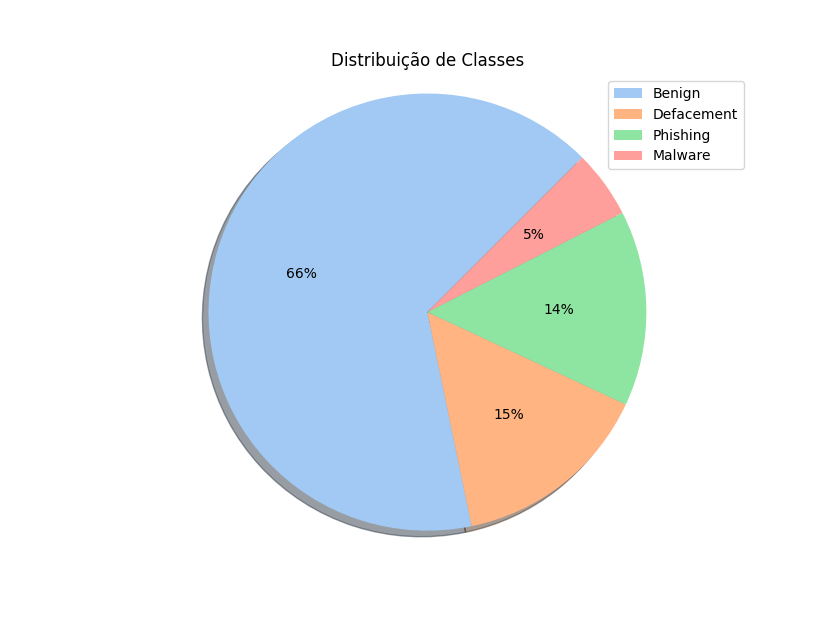
\includegraphics[width=0.95\textwidth]{pic/Figure_1.png}
        \label{fig:exampleFig1}
    \end{figure}
    
\end{frame}

\subsection{II. Comprimento das URLs}

\begin{frame}{Recapitulando}

    \begin{figure}[H]
        \centering
        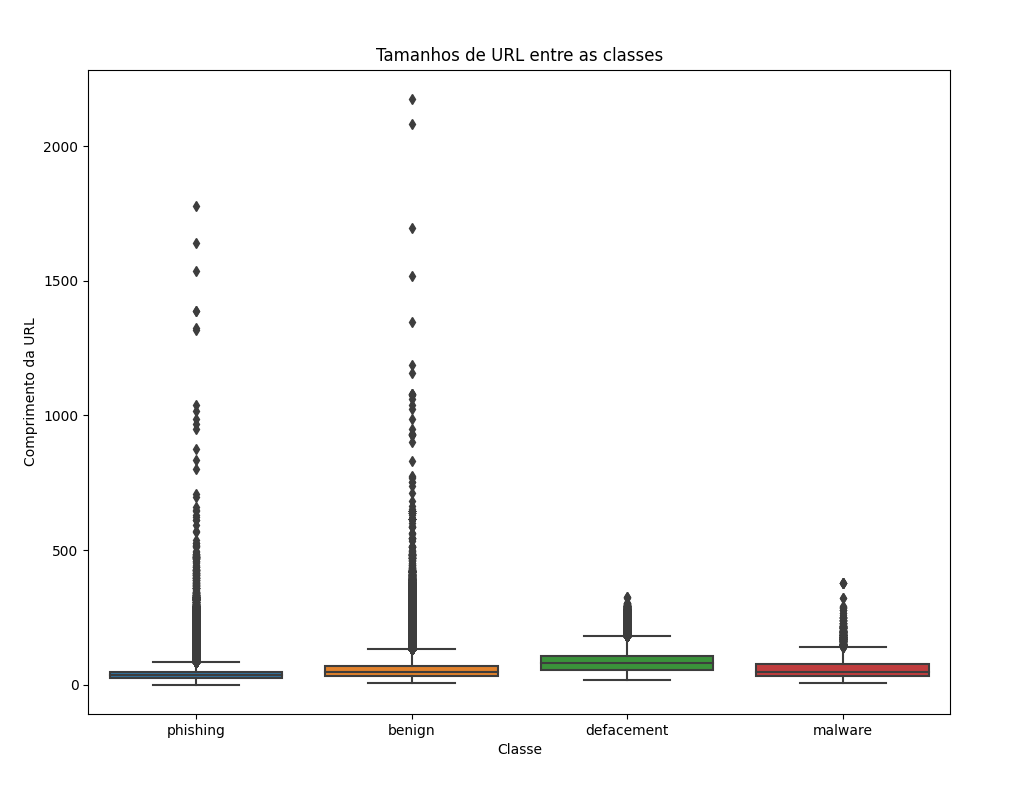
\includegraphics[width=0.85\textwidth]{pic/Figure_6.png}
        \label{fig:exampleFig2}
    \end{figure}
    
\end{frame}

\begin{frame}{Recapitulando}
    
    \begin{itemize}
        \item Equal-Frequency Binning
    \end{itemize}

    \begin{figure}[H]
        \centering
        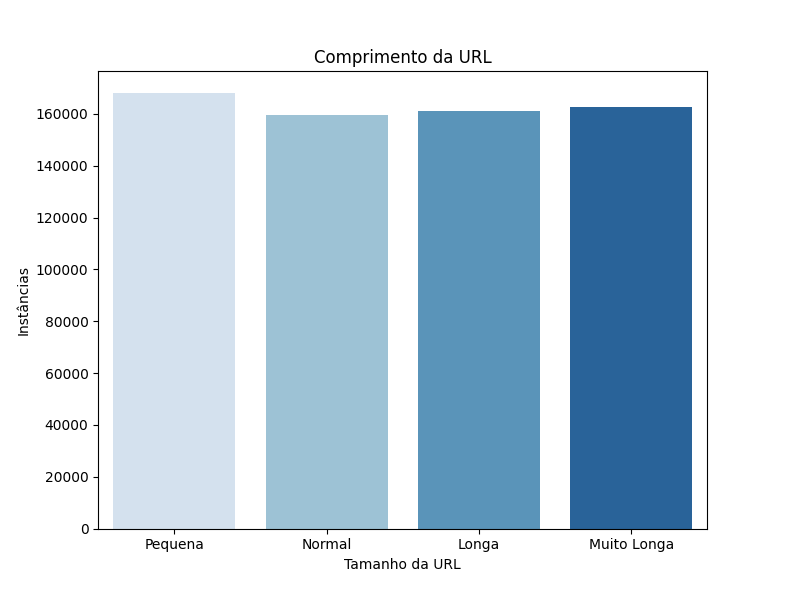
\includegraphics[width=0.8\textwidth]{pic/Figure_3.png}
        \label{fig:exampleFig3}
    \end{figure}
    
\end{frame}

\section{Análise Estatística}

\begin{frame}{Conteúdo} 
     \tableofcontents[currentsection]
\end{frame}

\begin{frame}{Estrutura de uma URL}

    \begin{figure}[H]
        \centering
        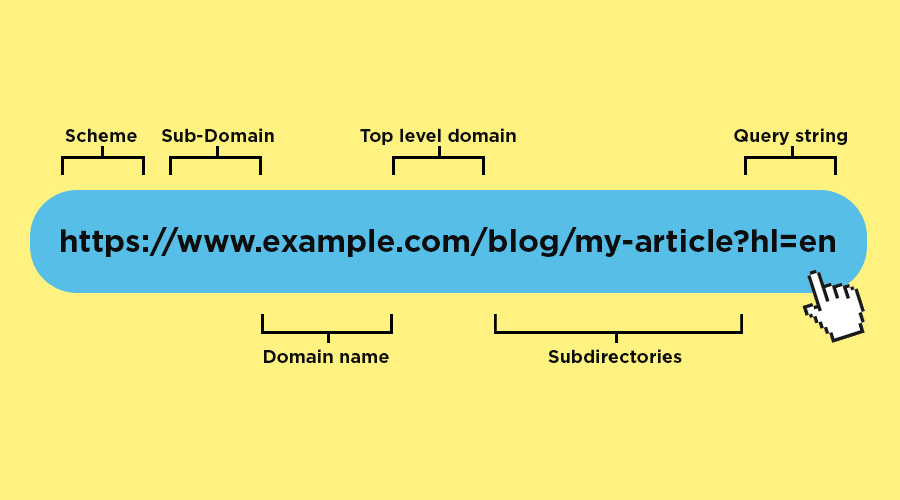
\includegraphics[width=0.9\textwidth]{pic/Diagram-of-a-URL.jpg}
        \label{fig:exampleFig4}
    \end{figure}
    
\end{frame}

\begin{frame}{Tipos de Caracteres}

    \begin{itemize}
        \setlength{\itemsep}{10pt}
        \item Disparidade na quantidade de caracteres não-alfanuméricos;
        \item Em relação às URLs seguras:
        \vspace{0.2cm}
        \begin{enumerate}
            \setlength{\itemsep}{10pt}
            \item URLs de \emph{defacement} possuem, em média, 75\% mais caracteres do tipo;
            \item URLs de \emph{malware} possuem, em média, o dobro de caracteres do tipo;
            \item URLs de \emph{phishing} possuem, em média, 25\% menos caracteres do tipo.
        \end{enumerate}
    \end{itemize}
    
\end{frame}

\section{Resultados Parciais}

\begin{frame}{Conteúdo} 
     \tableofcontents[currentsection]
\end{frame}

\begin{frame}{Matriz de Confusão}

    \begin{figure}[H]
        \centering
        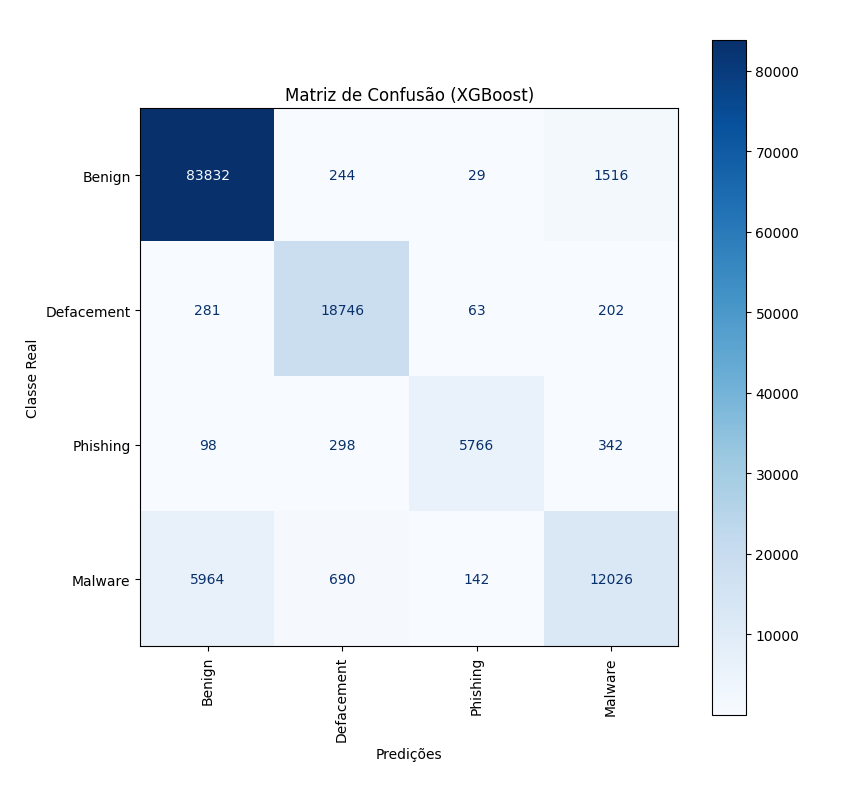
\includegraphics[width=0.75\textwidth]{pic/Figure_4.png}
        \label{fig:exampleFig9}
    \end{figure}
    
\end{frame}

\begin{frame}{F1 Score}

\begin{block}{}
\begin{table}
\centering

\resizebox{\columnwidth}{!}{
\begin{tabular}{|c|c|c|}

%\begin{tabularx}{\columnwidth}{|lcccc|}
\hline 
 
\multicolumn{3}{|c|}{TP 1}\\ 
\hline 

 Algoritmo & Média  & Desvio Padrão\\
 \hline 
 %\rowcolor{Gray}
%\multicolumn{5}{|c|}{Dictionary} \\ 
% \hline 
Regressão Logística & 0,4343240025832924 & 0,0014418608790156475\\   %\hdashline
XGBoost & 0,8218246353658317 & 0,001907892449405127\\  %\hdashline 
  \hline 


\end{tabular}
}
%\end{tabularx}
%\label{se:Dic}
\end{table}
\end{block}
\note[item]{.}


\begin{block}{}
\begin{table}
\centering

\resizebox{\columnwidth}{!}{
\begin{tabular}{|c|c|c|}

%\begin{tabularx}{\columnwidth}{|lcccc|}
\hline 
 
\multicolumn{3}{|c|}{TP 2 - Parcial I}\\ 
\hline 

 Algoritmo & Média  & Desvio Padrão\\
 \hline 
 %\rowcolor{Gray}
%\multicolumn{5}{|c|}{Dictionary} \\ 
% \hline 
Regressão Logística & 0,5780295368328738 & 0,0021293237223429956\\   %\hdashline
XGBoost & 0,8568910936179079 & 0,0017065729226258411\\  %\hdashline 
  \hline 


\end{tabular}
}
%\end{tabularx}
%\label{se:Dic}
\end{table}
\end{block}
\note[item]{.}

\end{frame}

\section{Próximos Passos}

\begin{frame}{Conteúdo} 
     \tableofcontents[currentsection]
\end{frame}

\begin{frame}{Finalização da Parcial I}

    \begin{itemize}
        \setlength{\itemsep}{10pt}
        \item Balanceamento da base:
        \begin{enumerate}
            \item PhishTank;
            \item Kaggle;
            \item \emph{Oversampling?}.
        \end{enumerate}
        \item Novos atributos:
        \begin{enumerate}
            \item Conteúdo das páginas;
            \item Dados de rede.
        \end{enumerate}
    \end{itemize}

\end{frame}

\begin{frame}{Parcial II}

    \begin{itemize}
        \setlength{\itemsep}{10pt}
        \item Seleção de 2 a 4 algoritmos mais recentes;
        \item Formulação do modelo com a base polida;
        \item Comparativo com trabalhos relacionados.
    \end{itemize}

\end{frame}

% \begin{frame}{Referências}
%     \scriptsize\bibliographystyle{apalike}
%     \bibliography{ref}
% \end{frame}

\end{document}